% !TEX root = Presentation.tex
% Change "draft" to "final" when you're done.
\documentclass[compress]{beamer}

% !TEX root = Thesis.tex
\usepackage{morewrites}									% Greedy packages...
\usepackage{fontspec}									% Use nicer system fonts
%\usepackage{mathdesign}
\usepackage{graphicx}									% Pretty pictures
\usepackage{todo}										% List of things to do
\usepackage{amsmath}									% Allow use of amsthm
\usepackage{amsthm}										% Pretty theorem environments
\usepackage{amssymb}									% More math symbols
\usepackage{algorithm}									% Pretty algorithm environment
\usepackage{algorithmic}								% Pretty algorithms
\usepackage[nounderscore]{syntax}						% BNF grammars
\usepackage{minted}										% Pretty code
\usepackage{tikz}										% Diagrams
\usepackage{booktabs}									% Pretty tables
\usepackage{nag}										% Complain
\usepackage[all]{xypic}									% Easy (compared to tikz) diagrams
\usepackage{unicode-math}								% Unicode symbols in math
\usepackage{caption}									% Possible del for subcaption
\usepackage{subcaption}									% Subfigures
\usepackage{forest}										% Simple trees
\usepackage{subdepth}
\usepackage{comment}									% How is this not built-in?
\usepackage{varioref}
\usepackage[linktocpage=true,colorlinks=true]{hyperref}	% Helpful links
\usepackage{cleveref}
\usepackage{datatool} % Import database tables

% Apparently must go after hyperref to get pretty links
\usepackage[acronym,style=tree]{glossaries}				% Glossary of terms

% Use and configure bibliography
\usepackage[backend=biber,style=trad-alpha]{biblatex}
\addbibresource{Thesis.bib}

% Define a new environment for Clojure code
\newmintedfile[cljcode]{clj}{linenos,frame=topline,frame=lines,framesep=2mm}
% SQL too!
\newminted{sql}{linenos,frame=topline,frame=lines,framesep=2mm}

% Configure tikz for pretty diagrams
\input tikz
\usetikzlibrary{fit}

% For some reason using minted with tikz causes minted to fail to colourize
% the output.  Should find a solution later, not really important right now.
\usemintedstyle{bw}

% Define new theorem environments
\theoremstyle{definition}
\newtheorem{defn}{Definition}
\newtheorem{ex}{Example}
\newtheorem{remark}{Remark}
\newtheorem{claim}{Claim}

% Change the image path prefix
\graphicspath{{images/}}

% Make the text worth looking at
\defaultfontfeatures{Ligatures=TeX}
\setmainfont[
	Kerning=Uppercase
]{Garamond Premier Pro}
\setmathfont{XITS Math}
\setmathfont[range=\mathbfsfit/{greek,Greek,latin,Latin}]{Garamond Premier Pro}
\setmonofont[Scale=0.9]{Consolas}

%\todo{Figure out why EB Garamond doesn't bold definitions}

% amsldoc, Section 4.14.2
\providecommand{\abs}[1]{\lvert#1\rvert}
\providecommand{\norm}[1]{\lVert#1\rVert}

% Simplify some of our function declarations
\DeclareMathOperator{\similarity}{similarity}
\DeclareMathOperator{\df}{df}
\DeclareMathOperator{\tfidf}{tf-idf}
\DeclareMathOperator{\tf}{tf}
\DeclareMathOperator{\idf}{idf}
\DeclareMathOperator{\score}{score}
\DeclareMathOperator{\freq}{freq}
\DeclareMathOperator{\query}{query}

% Expect the function name and any arguments separated by commas
\newcommand{\prop}[2]{\ensuremath\textsc{#1}\bigl[#2\bigr]}
% Expect the relation name and command-separated list of attributes
\newcommand{\rel}[2]{\ensuremath\mathrm{#1}\bigl(\mathrm{#2}\bigr)}

\newcommand{\relation}{\ensuremath r}
\newcommand{\tuple}{\ensuremath t}
\newcommand{\term}{\ensuremath \tau}
\newcommand{\field}{\ensuremath f}
\newcommand{\attribute}{\ensuremath \alpha}
\newcommand{\key}{\ensuremath \Kappa}
\newcommand{\db}{\ensuremath \mathbb{D}}
\newcommand{\doc}{\ensuremath d}
\newcommand{\dc}{\ensuremath \mathbb{C}}
\newcommand{\terms}{\ensuremath \Tau}
\newcommand{\q}{\ensuremath q}
%\newcommand{\sgraph}{\ensuremath G}
\newcommand{\egraph}{\ensuremath G}

\newcommand{\relations}[1]{\prop{Rel}{#1}}
\newcommand{\attributes}[1]{\prop{Attr}{#1}}
\newcommand{\fields}[1]{\prop{Field}{#1}}
\newcommand{\name}[1]{\prop{Name}{#1}}
\newcommand{\keys}[1]{\prop{Key}{#1}}
\newcommand{\fks}[1]{\prop{FK}{#1}}
\newcommand{\bag}[1]{\prop{Bag}{#1}}
\newcommand{\docs}[1]{\prop{Doc}{#1}}
\newcommand{\sgraph}[1]{\prop{SchemaGraph}{#1}}
\newcommand{\uid}[1]{\prop{UID}{#1}}
%\newcommand{\terms}[1]{\fcn{Term}{#1}}

% Use booktabs for datatool tables
% Stolen from SO:  http://tex.stackexchange.com/a/128581
\renewcommand{\dtldisplaystarttab}{\toprule}
\renewcommand{\dtldisplayafterhead}{\midrule}
\renewcommand{\dtldisplayendtab}{\\\bottomrule}

% Load databases
\DTLloaddb{db-link}{../../project/data/superheroes/Link.csv}
\DTLloaddb{db-person}{../../project/data/superheroes/Person.csv}
\DTLloaddb{db-superhero}{../../project/data/superheroes/Superhero.csv}
\DTLloaddb{db-planet}{../../project/data/superheroes/Planet.csv}

\newglossary{symbols}{sym}{sbl}{List of Symbols}
\makeglossaries

\includeonly{data-model,have-it-all,along-came-clojure,evaluation}

%\usetheme{Frankfurt}
%\usecolortheme{lily}

\definecolor{uoit-light-blue}{RGB}{0,119,202}
\definecolor{uoit-dark-blue}{RGB}{0,60,113}

\definecolor{UniBlue}{RGB}{83,121,170}
%\setbeamercolor{title}{fg=UniBlue}
%\setbeamercolor{frametitle}{fg=UniBlue}

%\setbeamercolor{primary text}{fg=uoit-dark-blue}
%\setbeamercolor{palette primary}{fg=uoit-dark-blue}
\setbeamercolor{palette tertiary}{fg=uoit-light-blue}
\setbeamercolor{structure}{fg=uoit-light-blue}
\setbeamercolor{alerted text}{fg=uoit-light-blue}

%\setbeameroption{show notes}

\setbeamertemplate{footline}[frame number]

\newcommand{\prop}[2]{\ensuremath\textsc{#1}[#2]}

\newcommand{\attributes}[1]{\prop{Attr}{#1}}
\newcommand{\fields}[1]{\prop{Field}{#1}}
\newcommand{\uid}[1]{\prop{UID}{#1}}

\newcommand{\attribute}{\alpha}
\newcommand{\tuple}{t}
\newcommand{\doc}{d}
\newcommand{\field}{f}
\newcommand{\egraph}{T}

\title[M.Sc. Thesis -- \insertframenumber/\inserttotalframenumber]{Towards a Concurrent Implementation of Keyword Search Over Relational Databases}
\subtitle{M.Sc. Thesis}
\author[\copyright 2014 Richard Drake]{Richard Drake \\ \vspace{0.3em} \scriptsize{\texttt{richard.drake@uoit.ca}} \\ \vspace{1em} \tiny Supervisor:  Dr. Ken Q. Pu}
\institute[UOIT]{University of Ontario Institute of Technology \\ Oshawa, Ontario, Canada}
\date{\tiny 9 June 2014}

\usefonttheme{serif}

\begin{document}
	%\newacronym{rdbms}{RDBMS}{relational database management system}
\newacronym{sql}{SQL}{structured query language}
\newacronym{tfidf}{TF-IDF}{term frequency and inverse document frequency}
\newacronym{fk}{FK}{foreign key}
\newacronym{json}{JSON}{JavaScript object notation}
\newacronym{csv}{CSV}{comma-separated values}
\newacronym{stm}{STM}{software transactional memory}
\newacronym{jvm}{JVM}{Java virtual machine}
\newacronym{jdbc}{JDBC}{Java database connectivity}
\newacronym{dsl}{DSL}{domain-specific language}
\newacronym{api}{API}{application programming interface}
\newacronym{bfs}{BFS}{breadth-first search}
\newacronym{ff}{FF}{Ford-Fulkerson}

\newacronym{olap}{OLAP}{online analytical processing}
\newacronym{mdx}{MDX}{MultiDimensional eXpressions}
\newacronym{xml}{XML}{Extensible Markup Language}
\newacronym{html}{HTML}{HyperText Markup Language}
	
	\frame{\maketitle}
	
	%- transformation from relational to document model
	%- reversibility of the transformation
	%- the flexibility of the document model (spelling correction + entity group search)
	%- using document model to perform graph based search
	
	\section{Introduction}
		\begin{frame}{Motivation}
			\begin{itemize}
				\item Two important data models:
					\begin{itemize}
						\item The \alert{relational model} is rigid in structure and highly normalized
						\item The \alert{document model} is flexible and provides keyword search
					\end{itemize}
				\item Choice between data \alert{integrity} and \alert{accessibility}
				\item Why can't we have both?
			\end{itemize}
		\end{frame}
		
		%\begin{frame}{Data Model Evolution}
		%	\begin{itemize}
		%		\item Structured Data (1970 -- 2000)
		%			\begin{itemize}
		%				\item Relational databases
		%			\end{itemize}
		%		\item Textual Data and Keyword Search (1970 -- Present)
		%			\begin{itemize}
		%				\item Natural language
		%			\end{itemize}
		%		\item Semi-Structured Data (1990 -- 2010)
		%			\begin{itemize}
		%				\item Well-formed natural language
		%			\end{itemize}
		%		\item Hybrid Data Model (2010 -- Present)
		%			\begin{itemize}
		%				\item Mixture of structured and unstructured data
		%			\end{itemize}
		%	\end{itemize}
		%\end{frame}
	
	%\section{Background}
	
	%\section{Approach}
		\begin{frame}{Thesis Statement}
			\begin{quotation}
				A system could be built that is capable of \alert{transforming data from the relational model to the document model}.  The transformation is \alert{reversible}, allowing the original data model to be recovered.  This system would use the \alert{keyword search} capabilities, along with the \alert{relational information}, to quickly \alert{discover related fragments of information}.
			\end{quotation}
		\end{frame}
		
		\begin{frame}{Research Goals}
			\begin{itemize}
				\item Define a \alert{formal framework} for transforming data from the relational to document model
				\item Design a collection of expressive \alert{query operators} for analyzing text from relational data sets
				\item Perform \alert{graph search} over the document model
				\item Investigate implementation techniques to make the query operators performant on modern, \alert{multicore machines}
			\end{itemize}
		\end{frame}
		
		\begin{frame}{Relational Model}
			\begin{itemize}
				\item A \alert{database} is a collection of relations
				\item A \alert{relation} is a set of named tuples
				\item Each \alert{named tuple} consists of a set of attributes corresponding to values
				\item An \alert{entity group} is a set of related tuples (joined by foreign key constraints)
			\end{itemize}
		\end{frame}
		
		\begin{frame}{Document Model}
			\begin{itemize}
				\item A \alert{document collection} is a set of documents
				\item A \alert{document} may have one or more fields
				\item A \alert{field} is a bag of tokens
				\item A prescribed lexical \alert{analyzer} converts bodies of text into a bag of \alert{tokens}
			\end{itemize}
		\end{frame}
	
	\section{Implementation}
		\begin{frame}{Framework Overview}
			\begin{itemize}
				\item Indexing
					\begin{enumerate}
						\item \alert{Iterate} over all named tuples in relational database
						\item \alert{Convert} each named tuple into a document
						\item \alert{Encode} relational information into one or more \alert{indexing document(s)}
					\end{enumerate}
				\item Search
					\begin{enumerate}
						\item \alert{Fuzzy value search} at the tuple-level
						\item \alert{Graph search} for connections among entity groups
					\end{enumerate}
			\end{itemize}
		\end{frame}
		
		\begin{frame}[fragile]{Iterate}
			\begin{itemize}
				\item Each entity and entity group defined in a configuration file
				\item Configuration specifies the SQL query to retrieve all entities from database
				\item This query is executed and each row is converted
			\end{itemize}
			
			\begin{figure}
				\begin{verbatim}
  (crawl
    [this db-conn idx-w]
    (let [sql (S :sql)]
      (execute-query db-conn sql (fn [row] ...))))
				\end{verbatim}
				\caption{Code to iterate over every named tuple in entity group}
				\label{lst:crawl}
			\end{figure}
		\end{frame}
		
		\begin{frame}{Convert}
			\begin{itemize}
				\item Each attribute of a named tuple directly maps to a field in a document
				\item Analysis is performed on each attribute before storing in a field
				\item The framework supports multiple analyzers
			\end{itemize}
			
			\begin{align}
				\attributes{\tuple} &\xrightarrow{analyzed} \fields{\doc} \\
				\attribute_1, \attribute_2, \dotsc, \attribute_n &\xrightarrow{analyzed} \field_1, \field_2, \dotsc, \field_n
			\end{align}
			
			Where \(\alpha_i\) is the value of an attribute, and \(f_i\) are the resulting tokens in a document.
		\end{frame}
		
		\begin{frame}{Encode}
			\begin{itemize}
				\item Relational information between related named tuples is encoded in the \alert{indexing document}
				\item This document, \(x\), is the concatenation of unique identifiers of every related document
			\end{itemize}
			
			\begin{align}
				x[\text{``entities''}] = \left\{\uid{\tuple} : \tuple \in V(\egraph)\right\}
			\end{align}
			
			Where \(\egraph\) is the entity group, and \(V(\egraph)\) is the set of named tuples in the entity group.
		\end{frame}
		
		\begin{frame}{Fuzzy Search at Tuple-Level}
			The encoding allows us to perform the following:
			
			\begin{itemize}
				\item Fuzzy search of relational attributes
				\item Search of named tuples in relations
				\item Find entity groups
			\end{itemize}
		\end{frame}
		
		\begin{frame}[fragile]{Graph Search Over Document Space}
			\begin{itemize}
				\item Use the indexing document to discover adjacent nodes
				\item Issue search query to discover all entity groups containing \(\uid{u}\)
			\end{itemize}
			
			\begin{verbatim}
(boolean-query [[(query :type :group) :and]
                [(query :entities id) :and]])
			\end{verbatim}
		\end{frame}
		
		\begin{frame}{Graph Search Algorithm and Implementation}
			\begin{itemize}
				\item Chose \alert{Breadth-First Search (BFS)} as search algorithm
				\item Adapted BFS to run concurrently without locking using Clojure's \alert{Software Transactional Memory (STM)}
				\item Utilized Clojure's concurrency primitives (atoms, references) in the concurrent implementation of BFS
			\end{itemize}
		\end{frame}
	
	\section{Evaluation}
		\begin{frame}{Data Corpus}
			\begin{itemize}
				\item Derived from MyCampus data\footnote{\url{http://uoit.ca/mycampus/}}
			\end{itemize}
			
			\begin{footnotesize}
				\begin{table}
					\centering
					
					\begin{tabular}{ll}
						\toprule
						Relation & Attributes \\
						\midrule
						Course & \underline{code}, title, subject \\
						Section & \underline{id}, actual, campus, capacity, credits, levels, registration\_start, \\
						 & registration\_end, semester, sec\_code, sec\_number, year, course \\
						Schedule & \underline{id}, date\_start, date\_end, day, schedtype, hour\_start, hour\_end, \\
						 & min\_start, min\_end, classtype, location, section\_id \\
						Instructor & \underline{id}, name \\
						Teaches & \underline{id}, schedule\_id, instructor\_id, position \\
						\bottomrule
					\end{tabular}
					
					\caption{Subset of mycampus dataset schema}
					\label{tbl:schema}
				\end{table}
			\end{footnotesize}
		\end{frame}
		
		\begin{frame}{Benchmarking Queries}
			\begin{itemize}
				\item Keywords are sampled from the database to form search queries
					\begin{itemize}
						\item May not occur within the same entity group
						\item Sampled from instructor name, course code, section id, etc.
					\end{itemize}
				\item Search for connections between these keywords
					\begin{itemize}
						\item Must utilize graph search to discover connections between keywords
						\item Monitor distance (hops) between keywords and measure performance
					\end{itemize}
			\end{itemize}
		\end{frame}
		
		\begin{frame}{Results}
			\begin{figure}
				\centering
				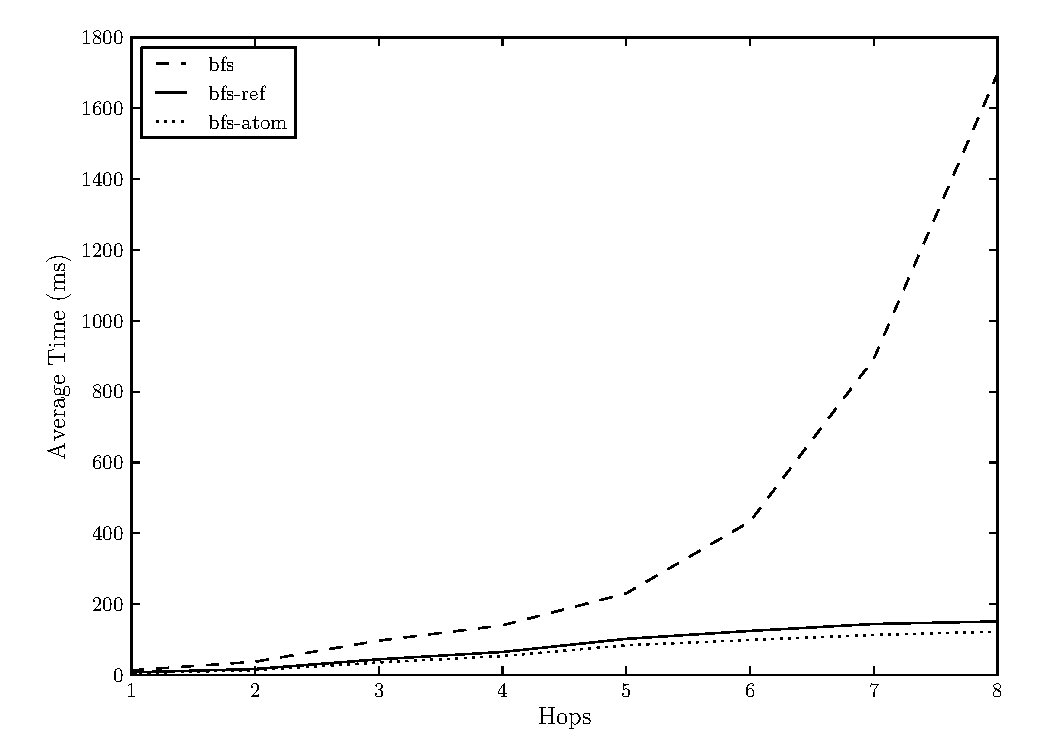
\includegraphics[scale=0.5]{../document/figures/charts/growth}
				\caption{Growth of runtime of each implementation, by hops}
			\end{figure}
		\end{frame}
		
		\begin{frame}{Results}
			\begin{figure}
				\centering
				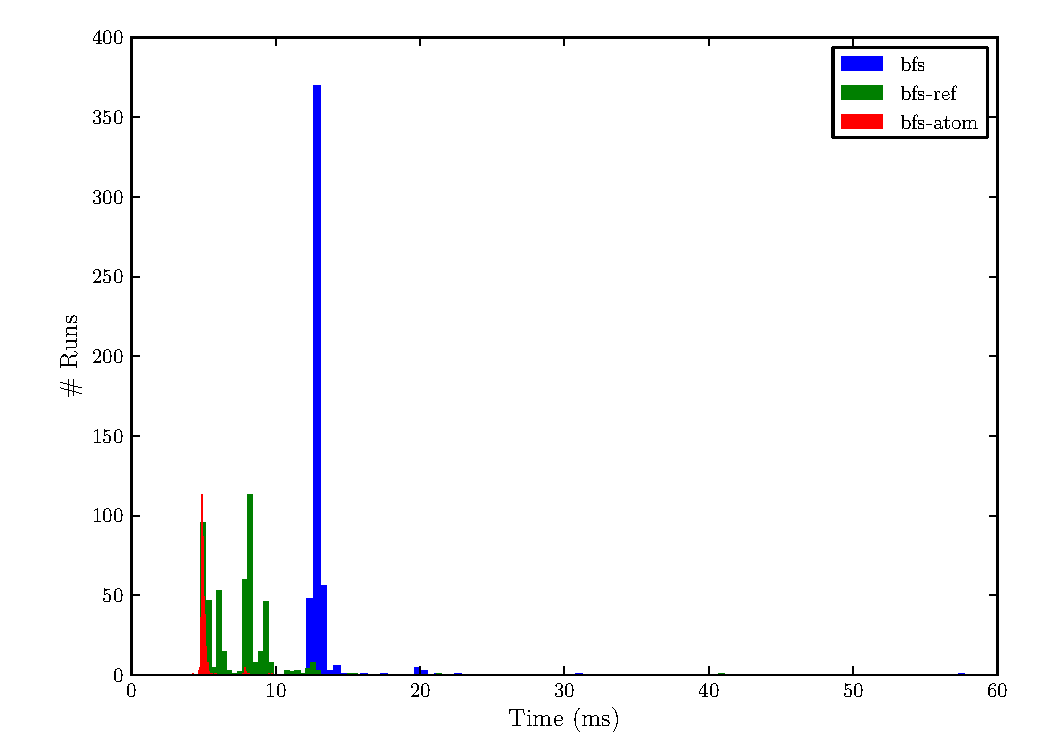
\includegraphics[scale=0.5]{../document/figures/charts/1_hops}
				\caption{Runtime of implementations, 1 Hop}
			\end{figure}
		\end{frame}
		
		\begin{frame}{Results}
			\begin{figure}
				\centering
				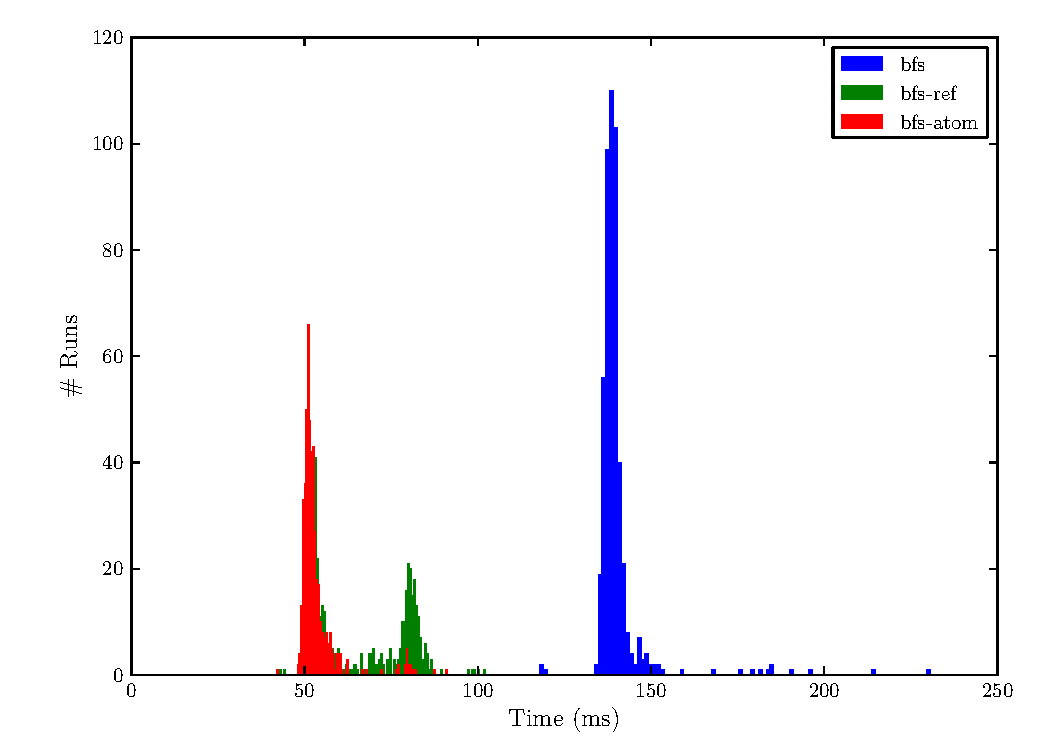
\includegraphics[scale=0.5]{../document/figures/charts/4_hops}
				\caption{Runtime of implementations, 4 Hops}
			\end{figure}
		\end{frame}
		
		\begin{frame}{Results}
			\begin{figure}
				\centering
				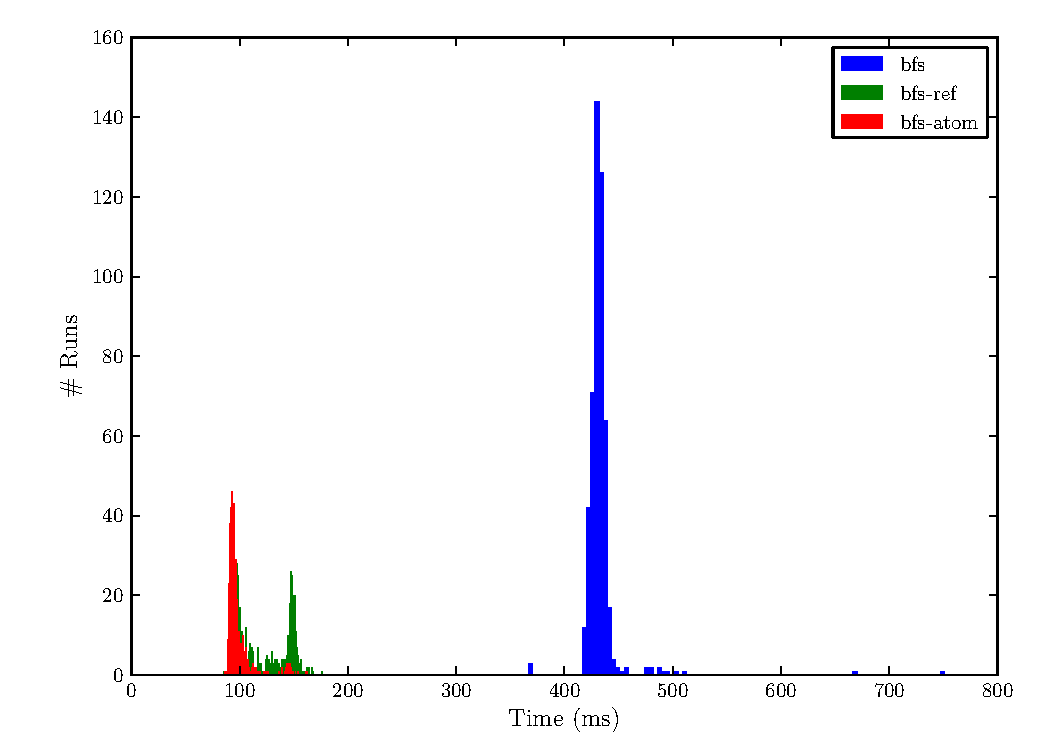
\includegraphics[scale=0.5]{../document/figures/charts/6_hops}
				\caption{Runtime of implementations, 6 Hops}
			\end{figure}
		\end{frame}
	
	\section{Conclusion}
		\begin{frame}{Contributions}
			\begin{itemize}
				\item Provided a framework to transform data from the relational to document model
				\item Demonstrated the reversibility of this transformation
				\item Utilized the flexibility of the document model
					\begin{itemize}
						\item e.g.~spelling correction, entity group search
					\end{itemize}
				\item Performed graph search over document space
				\item Investigated the reduction in runtime from a concurrent graph search
			\end{itemize}
		\end{frame}
		
		\begin{frame}{Lessons Learned}
			\begin{itemize}
				\item Simple algorithms are easiest to parallelize
				\item Clojure's STM implementation is simple and effective
				\item Clojure is powerful and encouraged correct code that was easier to optimize later
			\end{itemize}
		\end{frame}
		
		\begin{frame}{Publication}
			This work has been submitted to the 15th IEEE conference on Information Reuse and Integration.

			\begin{figure}
				\centering
				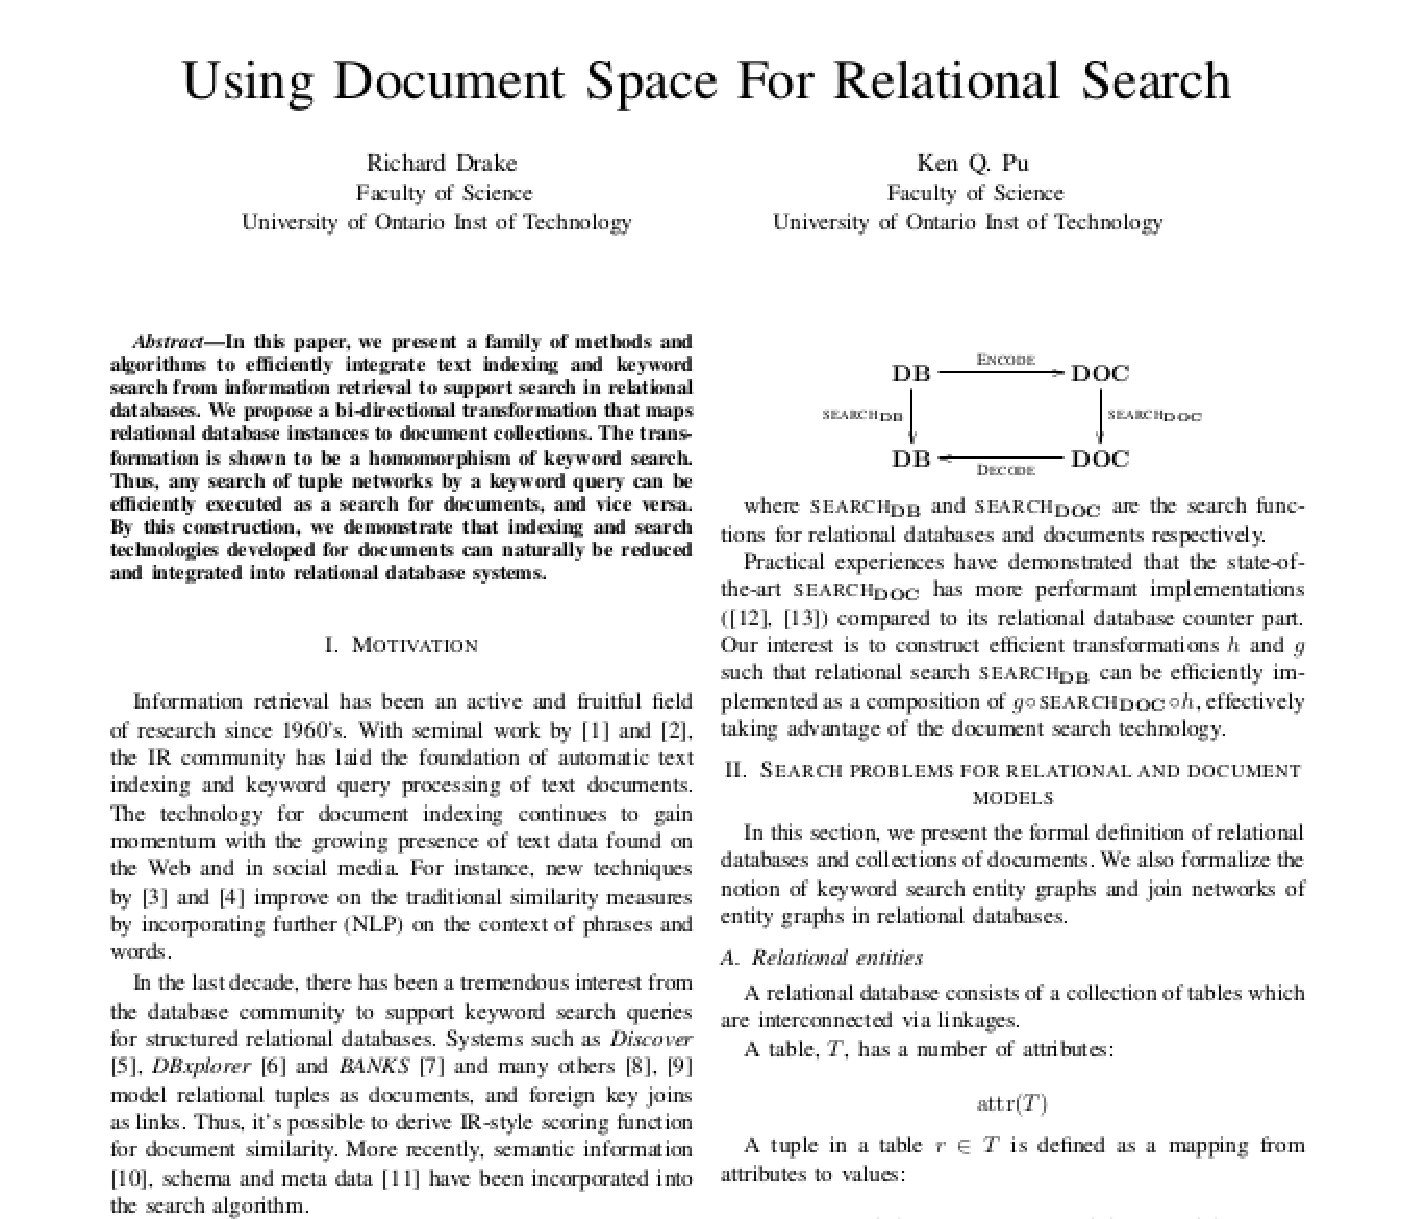
\includegraphics[scale=0.3]{paper-thumbnail}
			\end{figure}
		\end{frame}
		
		\begin{frame}{Future Work}
			\begin{itemize}
				\item Simplify configuration
				\item Incremental indexing
				\item Generalize results by benchmarking standard datasets
			\end{itemize}
		\end{frame}
	
	\section*{}
	
	\frame{\titlepage}
\end{document}
